\documentclass{anstrans} \usepackage{amsmath} \usepackage{amssymb}
%\usepackage{amsthm}
\usepackage{amscd}
%\usepackage{amsfonts}
\usepackage{graphicx}% \usepackage{fancyhdr} \usepackage{color} \usepackage{cite}

%\usepackage[T1]{fontenc} \usepackage[utf8]{inputenc} \usepackage{authblk}
\usepackage{physics} \usepackage{float} \usepackage{caption} \usepackage{subcaption}

\setlength{\columnsep}{0.5 in}

\newcommand{\expv}[1]{\ensuremath{\mathbb{E}[ #1]}} \newcommand{\xs}[2]{\ensuremath{\Sigma_{#1}^{(#2)}}}
\newcommand{\intO}{\ensuremath{\int\limits_{4\pi}}} \newcommand{\intz}{\ensuremath{\int\limits_0^1}}
\newcommand{\intf}{\ensuremath{\int\limits_{-\infty}^\infty}}
\newcommand{\intzf}{\ensuremath{\int\limits_{0}^\infty}}
\newcommand{\LargerCdot}{\raisebox{-0.25ex}{\scalebox{1.2}{$\cdot$}}}

%\textwidth6.6in \textheight9in


%\setlength{\topmargin}{0.3in} \addtolength{\topmargin}{-\headheight} \addtolength{\topmargin}{-\headsep}

%\setlength{\oddsidemargin}{0in}

%\oddsidemargin  0.0in \evensidemargin 0.0in \parindent0em

%\pagestyle{fancy}\lhead{MATH 579 (UQ for PDEs)} \rhead{02/24/2014} \chead{Project Proposal} \lfoot{}
%\rfoot{\bf \thepage} \cfoot{}
\title{Time-Dependent Sensitivity Analysis of OECD Benchmark using BISON and RAVEN}

\author{Paul W. Talbot$^{*\dagger}$, 
        Kyle Gamble$^{\ddagger}$,
        C. Rabiti$^{\dagger}$,
        C. Wang$^{\dagger}$, 
        A. Alfonsi$^{\dagger}$, 
        J. J. Cogliati$^{\dagger}$, 
        D. Mandelli$^{\dagger}$, 
        A. K. Prinja$^{*}$}
\institute{
  $^*$Department of Nuclear Engineering,
  University of New Mexico,
  Albuquerque, NM, 87131 
  \and 
  $^\dagger$Nuclear Engineering Methods Development,
  Idaho National Laboratory,
  Idaho Falls, ID, 83415
  \and
  $^\ddagger$Fuel Modeling and Simulation,
  Idaho National Laboratory,
  Idaho Falls, ID, 83415}
  \email{paul.talbot@inl.gov }%\and prinja@unm.edu \and cristian.rabiti@inl.gov}
%\date{}


\begin{document}
\section{Introduction}
Developments in uncertainty quantification for nuclear simulations have decreased the computational cost
required to perform accurate sensitivity analysis \cite{cristiansmeared,ans2014,ans2016sum,physor2016}.
This work demonstrates implementation of these methods in the RAVEN \cite{raven} framework,
allowing for time-dependent
sensitivity analysis.  By demonstration we consider an OECD benchmark case
\cite{OECDbench}.  We propagate uncertainties using RAVEN operating on the BISON
\cite{bison} fuels performance code.  We then consider the time-evolution of output response sensitivity
to uncertain inputs.  We perform sensitivity analysis  using time-based stochastic 
collocation for generalized polynomial chaos (SCgPC) and high-dimension model reduction (HDMR) \cite{Ayres}.
While uncertainty quantification applied to end-of-cycle statistics is useful, we demonstrate that dominant
sources of uncertainty for figures of merit may fluctuate throughout the simulation.  Time-dependent sensitivity
analysis allows more insight on key design parameters for fuel.

\section{Methods}
The details of the OECD benchmark and its parameter uncertainties are described in \cite{OECDbench}.
The benchmark includes a fuel pin in a steady-state PWR with power transients over a 2000 day period. During
this time there is a power ramp up, then two steps down in power.
Uncertain parameters include fuel properties, boundary conditions, and geometries.  We
treat each of the uncertain inputs as independent parameters and consider here four responses: maximum
centerline fuel temperature, maximum clad creep strain, fission gas
release percent, and clad elongation.  The input parameters and distributions are in Table
\ref{tab:unc}.
\begin{table}
  \centering
  \caption{Uncertain Parameters}
  \label{tab:unc}
  \begin{tabular}{c|c c | c}
  Parameter     & Mean     & Std. Dev.& Units   \\ \hline
  clad cond.    & 16       & 2.5      & W/m-K    \\
  clad thick    & 6.7e-4   & 8.3e-6   & m        \\
  clad rough    & 5e-7     & 1e-7     & m        \\
  creep rate    & 1        & 0.15     & s$^{-1}$ \\
  fuel cond.    & 1        & 0.05     & W/m-K    \\
  fuel dens.    & 10299.24 & 51.4962  & kg/m$^3$ \\
  fuel exp.     & 1e-5     & 7.5e-7   &          \\
  fuel radius   & 4.7e-3   & 3.335e-6 & m        \\
  fuel swell    & 5.58e-5  & 5.77e-6  &          \\
  gap cond.     & 1        & 0.025    & W/m-K    \\
  gap width     & 9e-5     & 8.33e-6  & m        \\
  mass flux     & 3460     & 57.67    & kg/m$^2$s\\
  rod pressure  & 1.2e6    & 4e4      & Pa       \\
  sys pressure  & 1.551e7  & 51648.3  & Pa       \\
  power scaling & 1        & 0.016667 &          \\ \hline
  Parameter     & Low      & High     & Units    \\ \hline
  inlet temp    & 558      & 564      & K
  \end{tabular}
\end{table}

For propagation of uncertainty we use the high-dimension model reduction (HDMR) expansion \cite{hdmr},
\begin{equation}\label{eq:hdmr}
  u(Y) = u_0 + \sum_{n=1}^N u_n + \sum_{n_1=1}^N\sum_{n_2=1}^{n_1-1} u_{n_1,n_2} + \cdots,
\end{equation}
where $u(Y)$ is the response as a function of inputs $Y=(y_1,\ldots,y_N)$, $N$ is the dimensionality of the
input space, and the components $u_i$ are defined as
\begin{equation}
  u_0 \equiv \int\cdots\int u(Y) \rho(Y) dY,
\end{equation}
\vspace{-10pt}
\begin{equation}
  u_1 \equiv \int\cdots\int u(Y) \rho(y_2,\cdots,y_N) dy_2\cdots dy_N,
\end{equation}
\vspace{-10pt}
\begin{equation}
  u_{1,2} \equiv \int\cdots\int u(Y) \rho(y_3,\cdots,y_N) dy_3\cdots dy_N,
\end{equation}
and so forth, where $\rho(Y)$ is the joint probability distribution function of $Y$.
Each of the terms in Eq. \ref{eq:hdmr} can be represented using a generalized polynomial chaos
expansion (gPC),
\begin{equation}
  u(Y) \approx \sum_{k\in\Lambda}c_k\Phi_k(Y),
\end{equation}
where $\Phi_k$ are multidimensional orthonormal polynomials of order $k=(k_1,\ldots,k_N)$ and $\Lambda$ is a
set
of multi-index polynomial orders.  Scalars $c_k$ are given using
sparse-grid collocation numerical integration \cite{smolyak},
\begin{equation}
  c_k = \int\cdots\int u(Y) \Phi_k(Y) \rho(Y) dY \approx \sum_{\ell=1}^L w_\ell u(Y_\ell) \Phi_k(Y_\ell).
\end{equation}

Sobol' sensitivity indices are obtained from HDMR expansion as \cite{sobolIndices}
\begin{equation}
  \mathcal{S}_i = \frac{\text{var}[u_i]}{\text{var}[u(Y)]}.
\end{equation}
The accuracy of Sobol' sensitivity indices depends on polynomial orders used in the subset
gPCs.  For this work, each subset is limited to first-order polynomials in
each dimension, providing linear global sensitivities.  While higher orders may reveal
additional features, the linear expansion is much less expensive to calculate and provides a reasonable
analysis of the uncertainty space.  For 17 inputs, only 34 BISON simulations were required, and the resulting
end-of-life statistics were in good agreement with previous studies for this benchmark \cite{dakotaBisonStudy}.

Time-dependent uncertainty analysis in RAVEN is performed using a snapshot approach: for each requested time
step through the simulation, a HDMR expansion surrogate model is created for each response using the data reported from BISON.
Interpolating between surrogates makes the collective time-dependent surrogate model.  In this mode, it is
critical to sample many time steps to provide accurate interpolation.  Because the quadrature points needed to
create the HDMR surrogates is the same at each time step, no additional BISON simulations are required to
transition from steady-state to time-dependent uncertainty analysis. Uncertainty analysis was recorded at 100
equally-spaced burnup points between the beginning and end of life.

\section{Results}\label{results}
The evolution of the mean and variance of the four responses over burnup is given in Figs. \ref{fig:mean}-\ref{fig:variance}. Each
response is scaled linearly by the parameter shown in the legend.  The nominal power shape in time is superimposed
for reference.  

From Figs. \ref{fig:centerline}-\ref{fig:elong} the variance generally increases as the transients are simulated; however, some drops in the
variance of the max centerline temperature warrant attention, in particular for Fig. \ref{fig:centerline}.  As
seen in Figs. \ref{fig:variance} and \ref{fig:centerline}, variance spikes for centerline temperature near
power changes in the transient.
As seen in Fig. \ref{fig:mean}, immediately after each power drop, the max
centerline temperature value drops significantly as well.  Because the variance is dominated by the system power
near the transients as shown in Fig. \ref{fig:variance}, the system power scaling factor is the chief source of variance.
Since the uncertain
parameter is a scaling factor, a reduction in the total power results in a smaller variance, which is
reflected in the reduction in variance for the max centerline temperature immediately after transients as per
Fig. \ref{fig:centerline}.  The peak in Fig. \ref{fig:elong} corresponds to the variance introduced by the
timing when the fuel expands to meet the clad.  Because this time is dependent on the initial gap thickness,
variance increases dramatically for the clad elongation depending on the thickness of the gap.
\begin{figure}[htb]
  \centering
  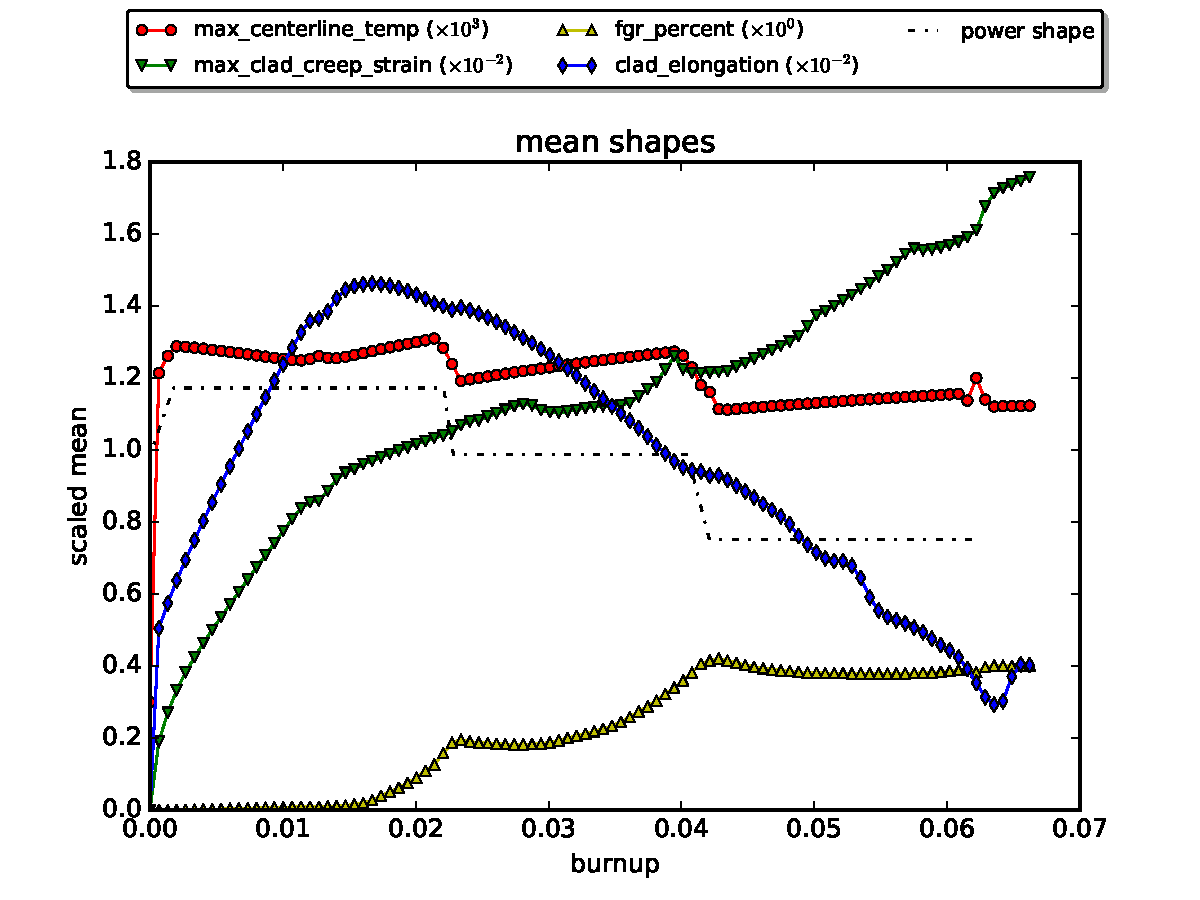
\includegraphics[width=\linewidth]{./meanplots}
  \caption{Response Mean Values}
  \label{fig:mean}
\end{figure}
\begin{figure}[htb]
  \centering
  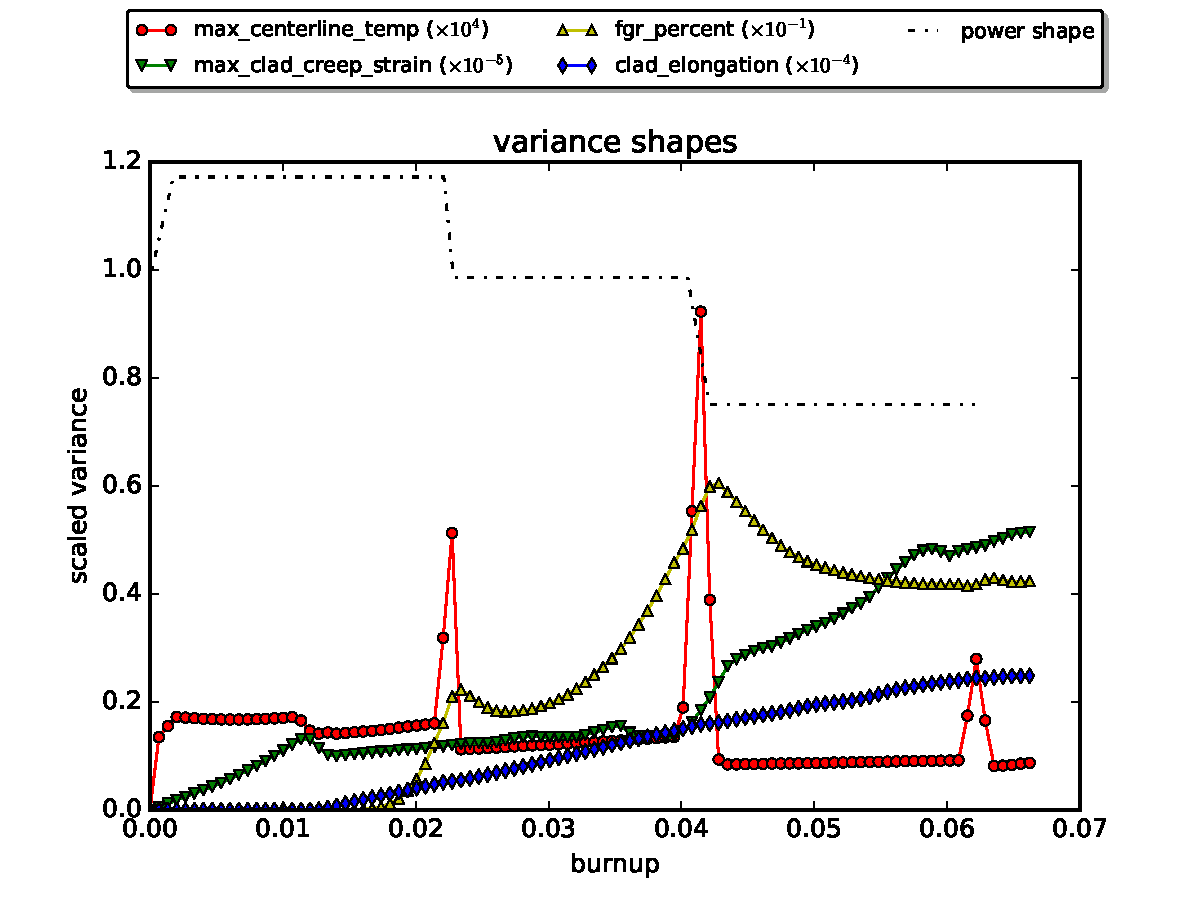
\includegraphics[width=\linewidth]{./varplots}
  \caption{Response Variance Values}
  \label{fig:variance}
\end{figure}

In Figs. \ref{fig:centerline}-\ref{fig:elong}, the evolution of sensitivities of various responses are shown
with respect to increasing burnup.  In addition, the power history used in the simulation is overlayed to
provide insight in time-based changes.  In each case, only the most significant uncertain inputs are shown
for clarity.  There are generally 4 significant events in the simulation cycle.  The first occurs just after
1\% fission per initial metal atom (FIMA), where the fuel has expanded enough to make contact with the clad.
The remainder are near 0.02, 0.04, and 0.06 FIMA, where the system power drops.

The max fuel centerline temperature is taken at the axial center of the fuel pin.  Sensitivity to the
fuel conductivity dominates over most of the variance history as seen in Fig. \ref{fig:centerline}; however, system
power has more impact near gradients in the power profile.
\begin{figure}[htb]
  \centering
  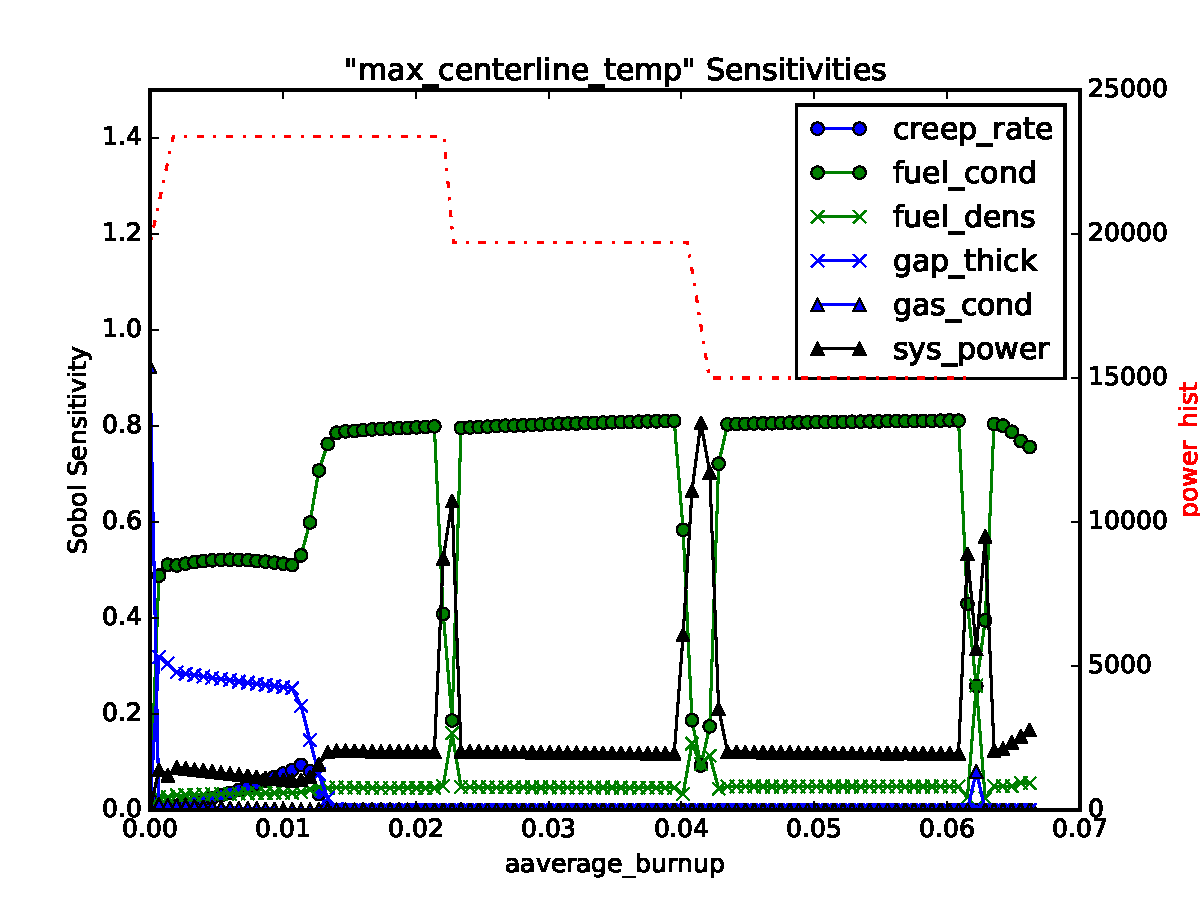
\includegraphics[width=\linewidth]{./sens_max_centerline_temp}
  \caption{Max Fuel Centerline Temperature}
  \label{fig:centerline}
\end{figure}

As expected, the clad creep rate is the most sensitive parameter for clad creep strain as shown in Fig.
\ref{fig:strain}; however, it is
interesting to note the rise and fall of the gap thickness as an important parameter in the middle of the
burnup range.
\begin{figure}[htb]
  \centering
  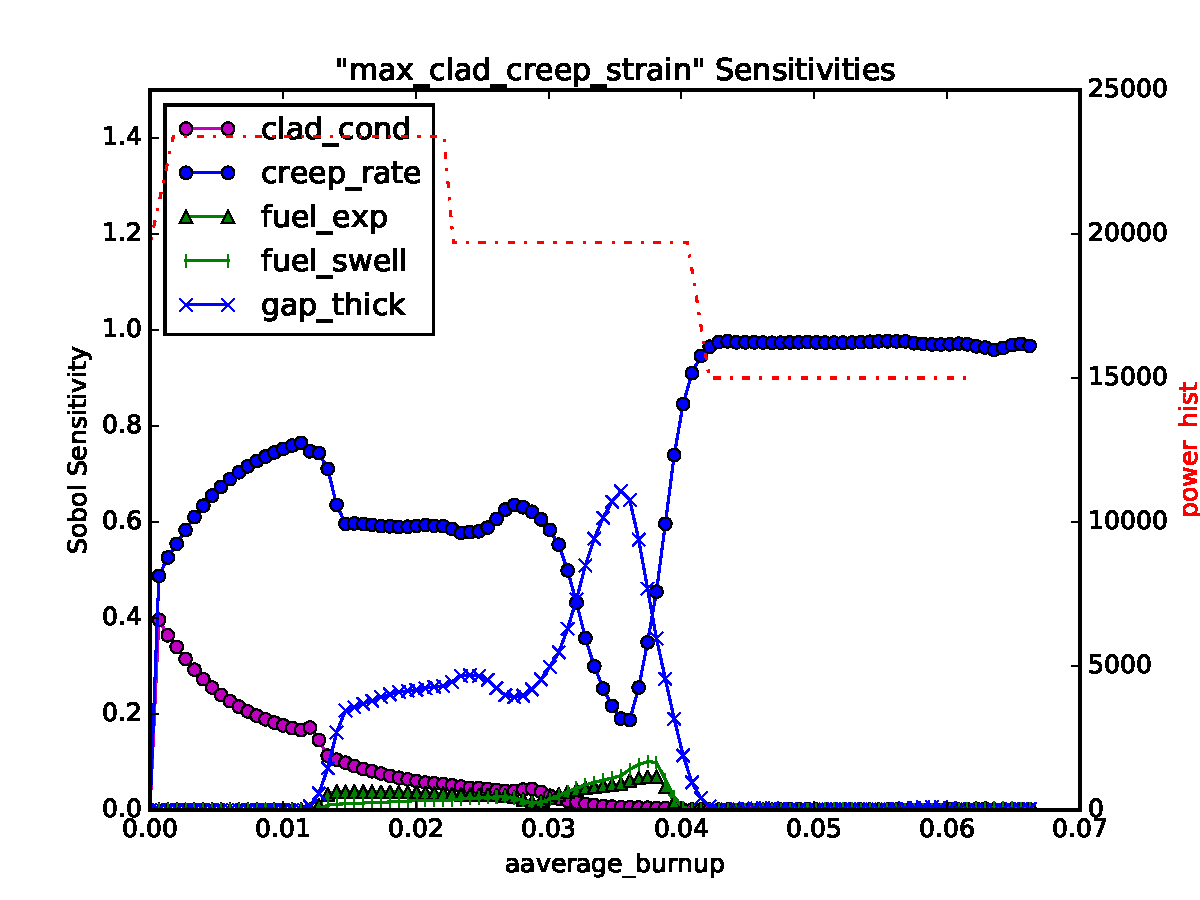
\includegraphics[width=\linewidth]{./sens_max_clad_creep_strain}
  \caption{Max Clad Creep Strain}
  \label{fig:strain}
\end{figure}

Early in life the fission gas release is dependent on several parameters, which gives way to only the fuel
conductivity and system power later.  This can be seen in Fig. \ref{fig:fgr}.
\begin{figure}[htb]
  \centering
  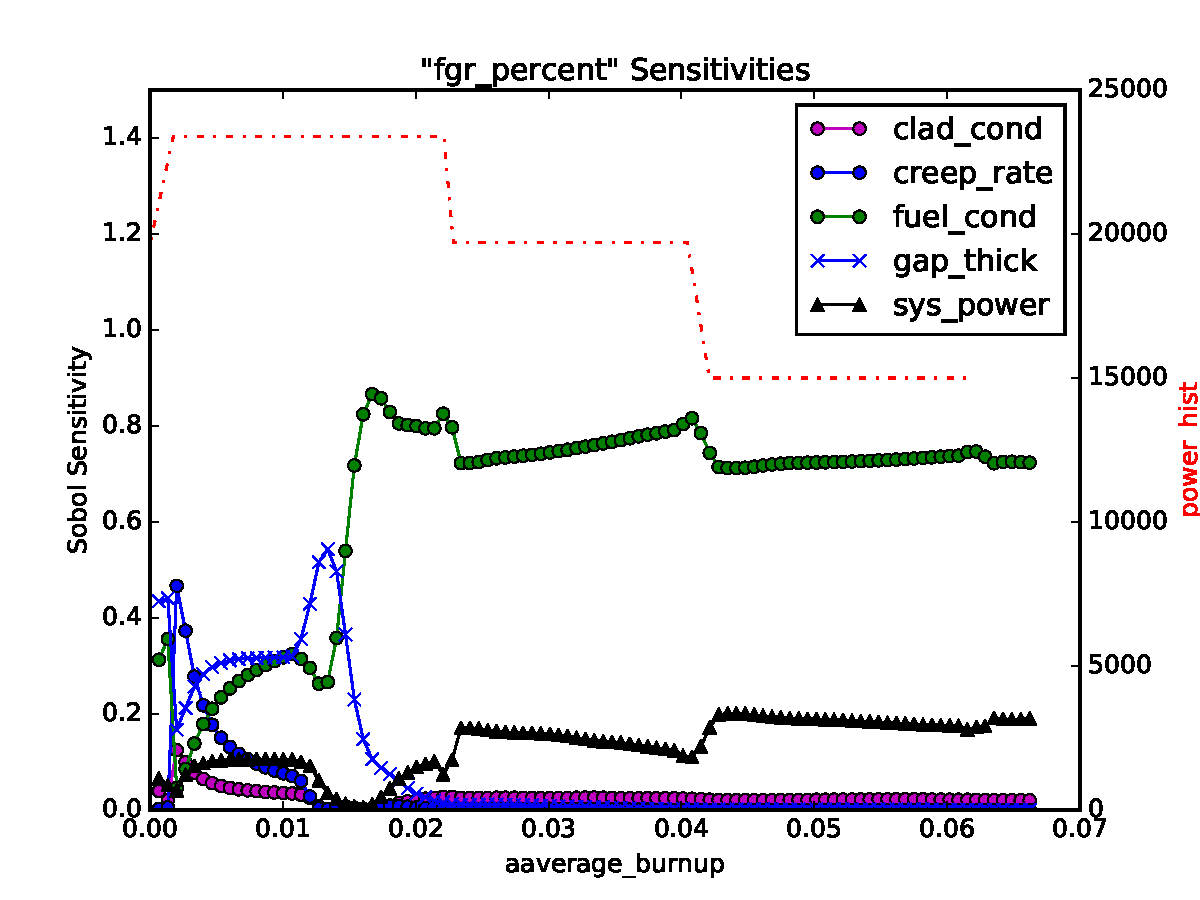
\includegraphics[width=\linewidth]{./sens_fgr_percent}
  \caption{Fission Gas Release (Percent)}
  \label{fig:fgr}
\end{figure}
The sensitivities in the variance of clad elongation have three distinct sections.  At the beginning, clad
elongation is perturbed most by clad conductivity, inlet temperature, and system power, with growing influence
from fuel density.  These are somewhat suddenly replaced by gap thickness, which then slowly trades places
with clad creep rate over the remainder of the life cycle.
\begin{figure}[htb]
  \centering
  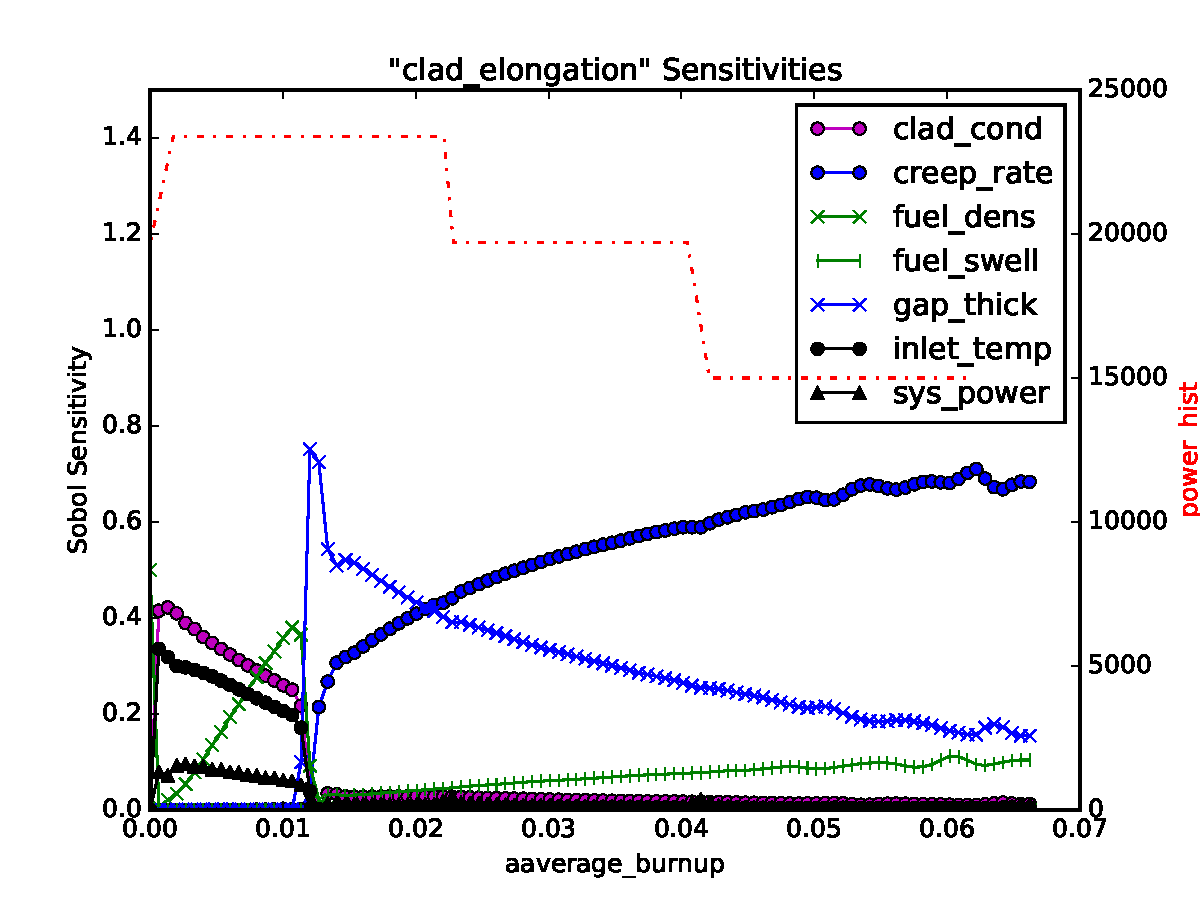
\includegraphics[width=\linewidth]{./sens_clad_elongation}
  \caption{Clad Elongation}
  \label{fig:elong}
\end{figure}

\section{Discussion}
We have demonstrated HDMR and SCgPC in RAVEN used to perform time-dependent uncertainty propagation
analysis in codes modeling transient behavior.  Reviewing the time-evolution of Sobol' sensitivities provides
new methods in understanding the impact of uncertain input parameters as changes occur during the transient
simulation.  At small additional cost to static uncertainty propagation, transient analysis has valuable
insights to offer.

\footnotesize
\bibliography{../bibliography/uq}{}
\bibliographystyle{ans}
\end{document}
